\PassOptionsToPackage{usenames, dvipsnames}{color}
\UseRawInputEncoding

\documentclass[12pt,usenames]{article}
\usepackage[a4paper, hmargin={2.8cm, 2.8cm}, vmargin={2.5cm, 2.5cm}]{geometry}  % Geometri-pakke: Styrer bl.a. maginer    %
%%%%%%%%%%%%%%%%%%%%%%%%%%%%%%%%%%%%%%%%%%%%%%%%%%%%%%%%%%%%%%%%%%%%%%%%%
\usepackage[en, nat, babel, titelside]{ku-forside} % KU-forside
\usepackage[utf8]{inputenc}
\usepackage[
backend=biber,
style=ieee,
sorting=ynt,
natbib=true
]{biblatex}
\addbibresource{bibliography.bib}

\usepackage{algpseudocode}
\usepackage{algorithm}

\usepackage{amsthm}
\usepackage{amsfonts}

\usepackage{mathtools}

\usepackage{float}

\usepackage{appendix}

\usepackage{graphicx}
\usepackage{caption}
\usepackage{subcaption}

\usepackage{hyperref}

\hypersetup{
    pdftitle={Parallel Bit-Counting for Approximate Similarity Searching},
    pdfpagemode=FullScreen,
}

\newtheorem{definition}{Definition}
\newtheorem{invariant}{Invariant}
\newtheorem{theorem}{Theorem}
\newtheorem{hypothesis}{Hypothesis}

\graphicspath{ {./assets} }

%
% Mini-manual til ku-forside pakken:
%
% Sprogmuligheder:     da, en
% babel loader babelpakken, med det valgte sprog
% Fakultetsmuligheder: farma, hum, jur, ku, life, nat, samf, sund, teo
% Farvemuligheder:     sh, farve
% Forsidemuligheder: lille, stor, titelside
%      titelside er identisk med designet på ku.dk/designmanual
%      lille er giver et lille logo sammen med titlen på den første side
%      stor er giver et stort logo sammen med titlen på den første side
%
% Default er [da,nat,farve,titelside]
%
% Ex. \usepackage[babel, lille, jur, sh, en]{ku-forside} giver et lille logo i sorthvid for juridisk fakultet og loader babelpakken med engelsk som sprog.

%%%%%%%%%%%%%%%%%%%%%%%%%%%%%%%%%%%%%%%%%%%%%%
%%%               Titel                    %%%
%%%%%%%%%%%%%%%%%%%%%%%%%%%%%%%%%%%%%%%%%%%%%%
\titel{Parallel Bit-Counting} %
\undertitel{for Approximate Similarity Searching} %
\opgave{Bachelor's project} % Findes kun under 'titelside'
\forfatter{Rasmus Hag Løvstad, \texttt{pgq596@alumni.ku.dk}}%
\dato{\today}%
\vejleder{Supervisor: Mikkel Thorup} %  Findes kun under 'titelside'
\begin{document}

% \title{Parallel Bit-Counting for Approximate Similarity Searching}
% \author{Rasmus Hag Løvstad}
% \date{Block 1+2, 2021}
\maketitle
% Spørgsmål:
% Hvilket problem omhandler denne artikel?
% Hvad prøver jeg at undersøge ved dette problem?
% Hvordan undersøger jeg dette?
% Hvad var mine konklusioner?
% Hvor sikre var disse?
\begin{abstract}
    % This project regards an analysis, implementation and comparison of existing efficient solutions to the Approximate Jaccard Similarity Search Problem of estimating the Jaccard Similarity between multiple sets. The findings include both a large theoretical and practical advantage of using advanced methods as presented by Dahlgaard et al.\cite{dahlgaard2017fast} and Knudsen\cite{fast-similarity-search} if the user is willing to pre-process the search-corpus before performing the search. This comparison both regards the precision of different methods as well as the run time of an real-world implementation. This is based on an implementation written in a low-level systems language and benchmarked on a regular personal computer with a statistical significance. Furthermore, reflections are made on how the results might scale on more specialized hardware.
    This project regards an analysis of recent advances in solving the Approximate Jaccard Similarity Search Problem, specifically in regards to how one can achieve sublinear query time using parallel bit counting as presented by Knudsen\cite{fast-similarity-search}. This contains a theoretical analysis of both runtime and correctness of the bit-counting algorithm as well as an empirical comparison to existing methods. The findings include both a theoretical and empirical run time advantage to using parallel bit counting compared to a simple, linear time algorithm. Furthermore, reflections are made on how the results might scale on more specialized hardware.
\end{abstract}

\tableofcontents
\section{Introduction}
The \textit{Approximate Similarity Search Problem} regards efficiently finding a set $A$ from a corpus $\mathcal{F}$ that is approximately similar to a query set $Q$ in regards to the \textit{Jaccard Similarity} metric $J(A,Q) = \frac{|A\cap Q|}{|A\cup Q|}$\cite{dahlgaard2017fast}\cite{fast-similarity-search}. Practical applications includes searching through large corpi of high-dimensional text documents like plagiarism-detection or website duplication checking among others\cite{vassilvitskii2018}. The main bottleneck in this problem is the \textit{curse of dimensionality}. Any trivial algorithm can solve this problem in $O(nd|Q|)$ time, but algorithms that query in linear time to the dimensionality of the corpus scale poorly when working with high-dimensional datasets. Text documents are especially bad in this regard since they often are encoded using \textit{$w$-shingles} ($w$ contigous words) which \citet{li2011hashing} shows easily can reach a dimensionality upwards of $d=2^{83}$ using just $5$-shingles.\\
The classic solution to this problem is the MinHash algorithm presented by \citet{broder1997minhash} to perform website duplication checking for the AltaVista search engine. It preprocesses the data once using hashing to perform effective querying in $O(n + |Q|)$ time, a significant improvement independent of the dimensionality of the corpus.
Many improvements have since been presented to both improve processing time, query time and space efficiency. Notable mentions includes (but are not limited to) the use of \textit{tensoring}\cite{andoni2006efficient}, \textit{b-bit minwise hashing}\cite{ping2011theory}, \textit{fast similarity sketching}\cite{dahlgaard2017fast}. Simple applications of these techniques leads to efficient querying with a constant error probability. If one wishes to achieve an even better error probability such as $\varepsilon = o(1)$, it is standard practice within the field to use $O(\log_2(1/\varepsilon))$ independent data structures and return the best result, resulting in a query time of $O(\frac{1}{\epsilon} (n^\rho + |Q|))$. Recent advances by \citet{fast-similarity-search} show that it is possible to achieve an even better query time by sampling these data structures from one large sketch. The similarity between these sub-sketches and a query set needs to be evaluated efficiently when querying, which requires efficient computation of the cardinality of a bit-string. To do this, \citet{fast-similarity-search} presents a general parallel bit-counting algorithm that computes the cardinality of a list of bit-strings in sub-linear time amortized due to word-parallism. This brings the query time down to $O((\frac{n\log_2 w}{w})^\rho \log(1/\varepsilon) + |Q|)$.\\
The main focus of this project is to analyse, prove, implement and evaluate this parallel bit-counting technique. The analysis will be based on the original paper \cite{fast-similarity-search}, but with some modifications to resolve some of the issues with the original algorithm. This will also include a pseudo-code implementation of the algorithm since the original paper only describes it through recurrences. This leads to a proof of correctness that slightly alters from the one presented in the paper, and a runtime analysis that does indeed show the sub-linear run time as claimed.\\
This theoretical analysis will be backed up by a real-life implementation that can be benchmarked to help show this sub-linear run time in practice. At last, reflections on the results and methods will be made to back up eventual conclusions.


\section{Theory}
% Hvad er Jaccard Similarity?
% Hvordan er problemet defineret fra et teoretisk perspektiv?
% Er der forskel i problemdefinitionerne? Hvad betyder dette for et sammenligningsperspektiv?
\subsection{Problem Definition}
The formal definition of the \textit{Jaccard Similarity Search Problem} is as follows:
Given a family $\mathcal{F}$ of $n$ sets from some universe $U$ and a query set $Q\subset U$, pre-process $\mathcal{F}$ to efficiently find the set $A\in \mathcal{F}$ such that $A = \max_{A\in \mathcal{F}}J(A,Q)$. \\
In many practical applications, it may be enough to only consider the \textit{Approximate Jaccard Similarity Search Problem} (as defined by \citet{fast-similarity-search}): Given the setting above and two constants $0 < j_2 < j_1 < 1$, pre-process $\mathcal{F}$ such that one can efficiently find some set $A \in \mathcal{F}$ such that $J(A,Q) \geq j_2$ if there exists some set $B \in \mathcal{F}$ where $J(B,Q) \geq j_1$. Note that it is possible for $A = B$. The intuition to this is that we can dial in how precise we expect our algorithm to be able to solve this problem by fine-tuning $j_2$ and $j_1$. We no longer expect the algorithm to return the \textit{best} solution, just one that is "good enough" (if a good solution exists). Algorithms that solve this problem should also be able to return "no answer", if no set $B\in \mathcal{F}$ upholds $J(B,Q)\geq j_1$, which is entirely possible depending on the parameters. \\
Most existing methods to solve this problem depend on the relationship between $j_1$ and $j_2$. This relationship is often described as $\rho=\frac{\log_2(1/j_1)}{\log_2(1/j_2)}$. Note that $\rho$ shrinks as $j_1$ approaches $1$. The query time of most solutions use $\rho$ as a exponent of $n$, which means that the lower the value of $\rho$ is, the fewer elements in the corpus needs to be checked.


\subsection{Trivial Solution}

% Broder's minhash som simpelt eksempel på en sketching-algoritme
% Forklaring om hvorfor det virker, samt dens asymptotiske køretid og lidt om dens præcision. Introducér en bound som vi kan sammenligne ud fra.
\subsection{MinHash}
The MinHash algorithm is one of the classic solutions to the \textit{approximate similarity search problem}, introduced by \citet{broder1997minhash} for the AltaVista search engine.\\
It is based on the following theorem:
\begin{theorem}
    \label{thm:minhash}
    Let $h$ be a universal hash function from $V \cup W \rightarrow [M]$ for some $M \in \mathbb{Z}^+$ where $W\cup V\subseteq U$ for some universe $U$. 
    Let $H(W)=\min_{w\in W} h(w)$. Then
    $$Pr[H(W)=H(V)]=\frac{|V\cap W|}{|V \cup W|}= J(V,W)$$
\end{theorem}
\begin{proof}
    If you sample a random element $x \in V \cup W$, then you can find the probability that $x \in V\cap W$ like so:
    $$Pr[x\in V \cap W]=\frac{|V\cap W|}{|V \cup W|}= J(V,W)$$
    When we calculate $H(W)$ and $H(V)$, the smallest value of the two will be $H(W\cup V)$. Since we use hash functions, this is essentially equivalent of sampling a random value from $W\cup V$. Assuming no collisions, this value will be in the intersection $W\cap V$ if and only if $H(W)$ and $H(V)$ have picked the same element. This means that the probability of $H(W)=H(V)$ is the same as the probability of picking an element of the intersection from the union, which is $\frac{|V\cap W|}{|V\cup W|}=J(V,W)$.
\end{proof}
The MinHash algorithm works like so: First, preprocess each set $A\in \mathcal{F}$ by hashing each coordinate using $k$ universal hash functions picked uniformly at random, saving the smallest value for each hash function as a sketch $S(A)=\langle H_0(A), \dots, H_{k-1}(A)\rangle$.
To query a set $Q$, calculate its sketch $S(Q)$ and then calculate $$d(S(A),S(Q))=\frac{1}{k}\sum_{i\in [k]}[H_i(A)=H_i(Q)]$$\\
We can then derive the expected value of this to be the Jaccard Similarity:
$$\mathbb{E}[d(S(A),S(Q))]=\mathbb{E}[\frac{1}{k}\sum_{i\in [k]}[H_i(A)=H_i(Q)]]$$
Using linearity of expectation:
$$=\frac{1}{k}\sum_{i\in [k]}\mathbb{E}[[H_i(A)=H_i(Q)]]$$
Using theorem \ref{thm:minhash}:
$$=\frac{1}{k}\sum_{i\in [k]}J(A,Q)$$
$$=J(A,Q)$$
% Since each hash function is independent, we can also use a Chernoff probability bound: Let us call each indicator variable $[H_i(A)=H_i(Q)]$ for $X_i$ and let $X=\sum_{i\in [k]}X_i$ and $\mu = \mathbb{E}[X]$. Then for any $\delta > 0$
% $$Pr[X > (1+\delta)\mu] < \left(\frac{e^\delta}{(1+\delta)^{(1+\delta)}}\right)^\mu$$
% $$Pr[X < (1-\delta)\mu] < \left(\frac{e^{-\delta}}{(1-\delta)^{(1-\delta)}}\right)^\mu$$
% The more hash functions we choose, the larger $k$ and $X$ will be, the larger $\mu$ will be and the stricter the bound will be. 
\subsubsection{Implementation with the LSH framework}
For a function $H\in \mathcal{H}$ from some family $\mathcal{H}$ defined as $H(W)=\min_{w\in W}h(w)$ as in theorem \ref{thm:minhash}, we know that $Pr[H(A)=H(B)]=J(A,B)$ as per theorem \ref{thm:minhash}. This must mean that $\mathcal{H}$ is $(j_1, j_2, j_1, j_2)$-sensitive for some values $0< j_2 < j_1 < 1$ as per definition \ref{thm:sensitive-hash} and theorem \ref{thm:minhash}:
\begin{itemize}
    \item If $J(W,V)\geq j_1$, then $Pr[H(W)=H(V)]\geq j_1$ 
    \item If $J(W,V) \leq j_2$, then $Pr[H(W)=H(V)] \leq j_2$.
\end{itemize}

We can then consider a function $g \in \mathcal{G}$ from some family $\mathcal{G}$ defined as $g(W) = \langle H_0(W), \dots, H_{k-1}(W) \rangle$ where functions $H_0 \dots H_{k-1}$ are picked uniformly at random from $\mathcal{H}$. An evaluation of any $g\in \mathcal{G}$ will be called a ``sketch'' from now on. Since the functions $H_0 \dots H_{k-1}$ are independent, we can use Bayes' theorem to derive that:
$$Pr[g(W)=g(V)] = Pr[\bigcap_{H \in g}H(W) = H(V)]$$
$$=\prod_{H\in g}Pr[H(W) = H(V)]$$
$$=\prod_{H\in g}J(W,V)=J(W,V)^k$$
This means that $\mathcal{G}$ is $(j_1, j_2, j_1^k, j_2^k)$-sensitive for some $k\in \mathbb{Z}^+$ since $J(W,V)$ and $j_1, j_2$ are non-negative:
\begin{itemize}
    \item If $J(W,V) \geq j_1$, then $J(W,V)^k \geq j_1^k$, which means that $Pr[g(W)=g(V)] \geq j_1^k$
    \item If $J(W,V) \leq j_2$, then $J(W,V)^k \leq j_2^k$, which means that $Pr[g(W)=g(V)] \leq j_2^k$
\end{itemize}
By choosing $k=\lceil \frac{\log_2(n)}{\log_2(1/j_2)} \rceil$, we can derive that $\mathcal{G}$ now is $(j_1, j_2, 1/n^\rho, 1/n)$-sensitive where $\rho=\frac{\log_2{1/j_1}}{\log_2{1/j_2}}$.
$$j_1^k = j_1^{\lceil\frac{\log_2(n)}{\log_2(1/j_2)} \rceil}\geq j_1^{\frac{\log_2(n)}{\log_2(1/j_2)}}$$
$$=j_1^{\frac{\log_2{(n)}}{\log_2{(1/j_2)}}\cdot\frac{\log_2{(1/j_1)}}{\log_2{(1/j_1)}}}$$
$$=j_1^{\frac{\log_2{(1/j_1)}}{\log_2{(1/j_2)}}\cdot-\frac{\log_2{(n)}}{\log_2{(j_1)}}}$$
$$=j_1^{-\rho\frac{\log_2{(n)}}{\log_2{(j_1)}}}$$
$$=j_1^{-\rho\log_{j_1}{(n)}}$$
$$=\frac{1}{n^\rho}$$
$$j_2^k\leq j_2 \cdot j_2^{\frac{\log_2(n)}{\log_2(1/j_2)}}=j_2\cdot j_2^{-\frac{\log_2{(n)}}{\log_2{(j_2)}}}=\frac{j_2}{n}\leq 1/n$$
%This has the consequence that both error probabilities ($r_1$ and $r_2$ from definition \ref{thm:sensitive-hash}) are dependent on $1/n$. 
Now, imagine $g_0, \dots g_{l-1} \in \mathcal{G}$ picked uniformly at random where $l=\lceil n^\rho \rceil$. If we calculate the sketch $g_i(A)$ for each $A\in \mathcal{F}$, $i\in [l]$, we will have $O(n\cdot l)$ sketches where $n=|F|$. This is our LSH data structure. \\
For each value $i\in [l]$, a hash table should also be created to look up a set stored at index $g_i(Q)$ for some query set $Q$ in constant time.
Furthermore, each set $A\in \mathcal{F}$ stored in this hashtable should have an associated hash table over its elements.\\
Creating the data structure takes $O(\sum_{A\in \mathcal{F}}|A| \cdot l)$ time and space during the preprocessing step.\\
To query, we first calculate $l$ sketches of $Q$, $g_0(Q), \dots, g_{l-1}(Q)$, which takes $O(k \cdot l \cdot |Q|)$ time. These sketches can be used to retrieve $l$ candidate sets $\mathcal{M} = \{ A_0, \dots A_{l-1}\}$ from each of the $l$ outermost hash tables. \\
For each $A\in \mathcal{M}$, the Jaccard similarity can be computed in $O(|Q|)$ time by computing the size of the intersection using the associated hash table to $A$ and computing the size of the union by the inclusion-exclusion principle if the size of $A$ is known.\\
When an element $A\in \mathcal{M}$ is found such that $J(A,Q) \geq j_2$, the algorithm can return.\\
This algorithm can therefore query in $O(l\cdot k |Q|\) = O(n^\rho\log_2{(n)}|Q|)$ time.
% Let us try to calculate how many of the candidate sets are so-called ``bad matches'' e.g. sets $A\in \mathcal{F}$ where $A \leq j_2$. Let $\mathcal{F}_{bad} = \{ A \in \mathcal{F} \mid J(A,Q) \leq j_2 \}$. Let $X_i(A) = [g_i(A) = g_i(Q)]$ for $i\in [l]$ and $A \in \mathcal{F}_{bad}$ and $X=\sum_{A \in \mathcal{F}_{bad}}\sum_{i\in [l]}X_i(A)$. Then we can calculate the expected amount of the $l$ sketches that contains a set $A\in \mathcal{F}_{bad}$.
% $$\mathbb{E}[X] = \mathbb{E}[\sum_{i\in [l]}\sum_{A \in \mathcal{F}_{bad}}X_i(A)] = \sum_{i\in [l]}\sum_{A \in \mathcal{F}_{bad}}\mathbb{E}[X_i(A)]$$
% Since $\mathcal{G}$ is $(j_1, j_2, 1/n^\rho, 1/n)$-sensitive, then $Pr[g_i(A) = g_i(Q)] \leq 1/n$ when $A\in \mathcal{F}_{bad}$:
% $$\leq \sum_{i\in [l]}\sum_{A \in \mathcal{F}_{bad}}1/n = \lceil n^\rho \rceil \cdot |\mathcal{F}_{bad}|\cdot 1/n \leq (n^{\rho - 1} + 1/n)|\mathcal{F}_{bad}| = $$
% We can try to compute the expected amount of bad matches. If a set $A \in \mathcal{F}$ exists such that $J(A,Q) \leq j_2$, we can be sure that it has at most a $1/n$ probability to get chosen as the candidate set for some $g_0 \dots g_{l-1}$, due to $g$'s $(j_1, j_2, 1/n^\rho, 1/n)$ sensitivity. Let $\mathcal{F}_{bad}$ denote the subset of $\mathcal{F}$ containing all the sets $A\in \mathcal{F}$ where $J(A,Q) \leq j_2$. Let a "bad match" denote a set $A\in \mathcal{F}$ where $J(A,Q) \leq j_2$ and $g(A) = g(Q)$, then we derive the following using linearity of expectation:
% $$E[\sum_{A\in \mathcal{F}_{bad}}[g(A) = g(Q)]]$$
% $$=\sum_{A\in \mathcal{F}_{bad}}E[[g(A) = g(Q)]]$$
% $$\leq \sum_{A\in \mathcal{F}_{bad}}1/n$$
% There can at most be $n=|F|$ bad matches:
% $$\leq n\cdot 1/n = 1$$
% We can therefore at most expect a constant amount of bad matches among the $l$ candidate sets.\\
% We can also calculate the expected amount of ``good matches'' if a set $A\in \mathcal{F}$ exists where $J(A, Q) > j_2$:
% Since $j_2 < j_1$, then:
% $$Pr[g_i(A) = g_i(Q)] \geq 1/n^\rho\quad \textrm{for any }i\in [l]$$
% $$\mathbb{E}[X]=\mathbb{E}[\sum_{i \in [l]}X_i] = \sum_{i \in [l]}\mathbb{E}[X_i] = \sum_{i \in [l]}Pr[g_i(A) = g_i(Q)] \geq l(\frac{1}{n^\rho}) = 1$$
% Therefore, we can expect at least constant amount of the $l$ candidate sets to be the set $A$.




% Since each of the $l$ functions are independent, we can then use the Chernoff bound with $\delta = \frac{1}{\mu}$:
% $$Pr[X \leq (1-\delta)\mu] \leq e^{-\frac{\delta^2\mu}{2}}$$
% $$\Leftrightarrow Pr[X \leq (1-\delta)] \leq e^{-\frac{\delta^2\mu}{2}}$$
% which can be converted to a constant error probability by keeping multiple independent data structures and returning the best result. By keeping $l=\lceil n^\rho \rceil$ different data structures, we reduce the error probability to $O(1)$.
% This means that the running time needed to create the required sketches is $O(l\cdot k \cdot |A|)=O(n^\rho \log_2(n)|A|)$ per data point $A \in \mathcal{F}$. The query time is now $O(l\cdot k \cdot |Q|)=O(n^\rho \log_2(n)|Q|)$ since we need to calculate a min-hash value of $|Q|$ for each of the $l$ sketches and look up a corresponding candidate set which takes $O(k\cdot |Q|)$ time per sketch. This process will lead to $l$ different candidate set, from which a true positive can be linearily searched in $O(l\cdot |Q|)$ time if a hash table has been created for each $|A|$ during the preprocessing step. This algorithm has a constant 1-sided error probability, since there is a constant probability that a set where $J(A,Q) > j_2$ hashes to a different value $g(A) \not = g(Q)$ and will therefore not be nominated as a candidate set. If the algorithm returns a set, we know that it for sure has $J(A,Q) \geq j_2$ however.

% Hvad er pointen med Fast Similarity Sketching
% Hvad har Dahlgaard introduceret? Hvordan gør de det sublineært? Hvad er de overordnede linjer for beviset?
% Hvad har Knudsen introduceret? Hvad er den teoretiske forskel?
\subsection{Fast Similarity Sketching}
Many improvements have since been discovered. The last step of each query of the LSH framework results in an expected $O(L)$ false positives that needs to be filtered out. By using an intermediate sketch of size $O(\log_2^3(n))$, it is possible to reduce the query time to $O((l\cdot |Q|)\log_2^3(n))$ by sampling from the intermediate sketch instead of the regular sketch \cite{dahlgaard2017fast}.
\citet{dahlgaard2017fast} have introduced an improved sketch, which is much faster to create and preserves the same properties as the MinHash sketch, while reducing the query time to $O(k\cdot l + |Q|)=O(n^\rho \log_2(n) + |Q|)$. Part of this improvement is due to a special algorithm that can eliminate bad matches by estimating if the Jaccard similarity between the query set and candidate set is above some threshold without calculating the actual Jaccard similarity. This reduces the filtering step to only take $O(l + |Q|)$ time, since the bad matches can be eliminated in $O(l)$ time and the amount of matches remaining is $O(1)$. \citet{christiani2018fast} has since improved this query time to $O(n^\rho + |Q|)$. \\
Until now, the data structures presented error with a constant probability $O(1)$. If one wants to reach a better error probability $1>\varepsilon>0$, it is common practice within the field to use $O(\log_2(1/\varepsilon))$ independent data structures. This will usually result in a query time of $O((n^\rho + |Q|)\log_2(1/\varepsilon))$. \\
\citet{fast-similarity-search} has shown a method of achieving an improved $O(n^\rho \log_2(1/\varepsilon)+|Q|)$ query time instead, which is very beneficial when working with highly dimensional datasets and a small $\varepsilon$. This is done by creating the $M$ different sketches of $Q$ nescessary for querying from one big sketch of size $M\cdot \log^3_2(n)$, with each sketch segment fed into each LSH datastructure.\\
\citet{fast-similarity-search} has further improved the query time to $O((\frac{n\log_2(w)}{w})^{\rho}\log_2(1/\varepsilon)+|Q|)$ by reducing $k$ such that $h_i\in \mathcal{H}$ becomes $(j_1, j_2, O((n/b)^\rho), n/b)$-sensitive where $b=w/\log_2w$ and then efficiently filtering through the $b$ expected "bad" matches. \\
Understanding why this filtering is efficient requires understanding the $b$-bit minwise hashing trick presented by \citet{li2011hashing}:
By only storing the $b$ lowest bits of each hash value, one can pack $O(\log_2(w)/b)$ hash values per word (where $w$ is the word size). \citet{fast-similarity-search} uses 1-bit minwise hashing to create a sketch of size $O(\log_2(w))$ per set $A\in \mathcal{F}$. This allows us to store $O(\frac{w}{\log_2(w)})$ sketches per word. \\
By calculating the amount of bits per sketch for $A$ and $Q$ that are equal, one can estimate the Jaccard Similarity to a degree which is good enough to filter a candidate match.\\
This calculation can be done by bitwise XOR'ing a word packed with sketches of different sets $A\in \mathcal{F}$ with a word packed with sketches of $Q$. Then, one can calculate the amount of bits set per word. Every bit set will then indicate that $Q$ and $A$ hashed to the same value, which means that we can filter each match based on whether or not the total amount of bits set is over some threshold.\\
It is this calculation on how to count these bits efficiently that the rest of this project will focus on.

\subsection{Parallel Bit Counting}
To be able to filter bad matches from good matches, we can use the 1-bit minwise hashing trick to pack the results of multiple subexperiments into one word, which by comparing the bit-wise cardinality (amount of bits set in a bit vector) of two words approximates the similarity between the two. % TODO: Research this!
One of the main techniques behind achieving an efficient run time of this method requires computing the cardinality of a bit vector efficiently. \citet{fast-similarity-search} presents a parallel algorithm to perform this but does neither describe any implementation details and has an unnecessarily complicated proof. I will try to describe the same algorithm in a much simpler fashion and prove its correctness and run time while doing it.
A naive algorithm to do this could be described like in algorithm \ref{alg:naive-cardinality}.
\begin{algorithm}[H]
\caption{A naive linear time algorithm}\label{alg:naive-cardinality}
\begin{algorithmic}[1]
\Function{Cardinality}{$w$, $d$} \Comment{$w$ is the input word, $d$ is the word-size}
\State $x \gets 0$
\State $i \gets 0$
\While{$i \leq d$}
\State $x \gets x + (w \gg i) \land 1$
\State $i \gets i + 1$
\EndWhile
\State \Return $x$
\EndFunction
\end{algorithmic}
\end{algorithm}
This algorithm trivially runs in linear time to the dimensionality $d$ of the input word $w$. For $n$ words of size $d$, this algorithm runs in $O(nd)$ time.
\citet{fast-similarity-search} presents two improvements to this: The first will improve the run time to $O(n\log(d))$ time by utilizing a divide-and-conquer technique and the second to $O(n + \log(d))$ time by introducing parallelism.
\subsubsection{Divide-and-Conquer}
To explain how divide-and-conquer methods can be used to improve run-time, we must first introduce a bit mask from \cite{fast-similarity-search} defined like so:
$$m_{i,j} = \underbrace{0\dots 0}_{2^{j}-2^{i}}\underbrace{1\dots 1}_{2^i}\dots\underbrace{0\dots 0}_{2^{j}-2^{i}}\underbrace{1\dots 1}_{2^i}$$
where $j > i$ and $j, i \in \mathbb{Z}^+$. The notation $m_{i}$ is a shorthand for $m_{i, i+1}$ and indicates a mask with an equal amount of 1's and 0's. By computing $w \land m_{i,j}$ for some word $w$ and some integers $i, j$, we can isolate a specific segments of size $2^i$ in the bitstring.
We will use this in the following operation:
\begin{equation}
    T(w, m, k) = (w\gg k) \land m
\end{equation}
This operation isolates the segments indicated by the bit-mask starting from the $k$th position of the word $w$.
The algorithm to calculate the cardinality can then be described like in algorithm \ref{alg:divide-and-conquer-cardinality}
\begin{algorithm}[H]
\caption{A divide-and-conquer approach}\label{alg:divide-and-conquer-cardinality}
\begin{algorithmic}[1]
\Function{Cardinality}{$w$, $d$} \Comment{$w$ is the input word, $d$ is the word-size}
\State $i \gets 0$
\While{$i \leq \log_2(d)$}
\State $w \gets T(w, m_i, 0) + T(w, m_i, 2^i)$
\State $i \gets i + 1$
\EndWhile
\State \Return $w$
\EndFunction
\end{algorithmic}
\end{algorithm}
The simplest way to gain intuition of this algorithm is to prove it. A loop-invariant is presented like so:
\begin{invariant}
\label{thm:divide-invariant}
At the $i$th iteration of the algorithm, each bitstring-segment of size $2^i$ of the word $w_i$ will contain the cardinality of the corresponding segment of the word $w_0$. Furthermore, the operation can be done in constant time.
\end{invariant}
\begin{proof}
    When $i=0$, then each bit-string of size $2^0=1$ in $w_0 = w$ will be $1$ if the bit is $1$ and $0$ if the bit is $0$. This proves our base case. \\
    If at step $i$ the word $w_i$ contains $\frac{d}{2^i}$ segments of size $2^i$, then invariant \ref{thm:divide-invariant} will be upheld if we combine each segment with it's neighbor to form a segment of size $2^{i+1}$. Since the cardinality of a combined bitstring is equal to the cardinality of its parts, we can divide all of the segments into pairs of size $2^{i+1}$ and add them together to form the new pair, which is done by the operation $T(w, m_i, 0) + T(w, m_i, 2^i)$ in constant time if the masks are pre-computed. This operation works because $T(w, m_i, 0)$ isolates every other segment of size $2^i$ starting from the first segment and $T(w, m_i, 2^i)$ isolates every other segment of size $2^i$ starting from the second segment.\\
\end{proof}
When the algorithm terminates after $\log_2(d)$ iterations, the segments will have size $2^{\log_2{(d)}} = d$ and thus span the entire original word, which means that we have the bit-count of the original word. % TODO: Skriv noget omkring hvad der sker når d ikke er en faktor af 2
\subsubsection{Parallelism}
To introduce parallelism into the algorithm, we must first realize the following: When two segments of $2^i$ bits gets combined, they will not need all of the $2^{i+1}$ bits to represent their sum. It is actually such that the bits used at iteration $i$ is exactly $i+1$.
\begin{invariant}
    At the $i$th iteration of the algorithm, the amount of bits set in a given segment of a word is at most $i+1$.
\end{invariant}
\begin{proof}
    We will prove this by induction. \\
    At $i=0$, the size of the segments are $2^0 = 1$, which is equal to $i+1$.\\
    If it is true at iteration $i$, then at iteration $i+1$ the algorithm will add two words of size $i+1$ which creates a word of size $i+2$, which fulfills the loop invariant.
\end{proof}
Now, we will introduce a function $l(i)$, which produces the smallest number such that $2^{l(i)} \geq i + 2$. If we use the bit mask $m_{l(i), i+1}$ instead of $m_{i}$, we will get the same result. This also means that we can pack $2^{i-l(i)}$ words into one by utilizing the empty space in each segment.
\begin{algorithm}[H]
\caption{A parallel divide-and-conquer algorithm}\label{alg:parallel-d-and-c}
    \begin{algorithmic}[1]
        \Function{Compute}{$S$, $d$} \Comment{$S$ is the input set, $d$ is the word-size}
            \State $n \gets S.length$
            \For{$i \in [\log_2(d)]$}
                \State $k' \gets \{\}$
                \State $t \gets \{\}$
                \For{$w \in S$}
                    \State $k' \gets k' \cup \{T(w, m_i, 0) + T(w, m_i, 2^i)\}$
                \EndFor
                \If{$i < 2$}
                    \State $S \gets k'$
                \Else
                \If{$l(i) = l(i+1)$}
                    \For{$j \in [\lceil S.length / 2 \rceil]$}
                    \State $t \gets t \cup \{k'_{2j} + (k'_{2j+1} \ll 2^i)\}$ % TODO: Er det l(i) eller l(i+1)?
                    \EndFor
                \Else
                    \For{$j \in k'$}
                        \State $t \gets t \cup \{T(k'_{j}, m_{l(i)}, 0) + (T(k'_{j}, m_{l(i)}, 2^{l(i)}) \ll 2^{i})\}$
                    \EndFor
                \EndIf
                \State $S \gets t$
                \EndIf
            \EndFor
            \State $S' \gets \{\}$
            \For{$j$ in $[S.length]$} \Comment{For every word in the final set}
            \For{$k$ in $[2^{l(\log_2(d))}]$} \Comment{For every original word embedded in $S_j$}% TODO: Research this!
                \State $S' \gets S' \cup \{T(S_j, m_{l(\log_2(d)), \log_2(d) + 1}, k\cdot 2^{l(\log_2(d))})\}$
                \EndFor
            \EndFor
            \State \Return $S'$
        \EndFunction
    \end{algorithmic}
\end{algorithm}
This algorithm is quite a bit more complex than the first one, and to prove it we need some more terminology.\\
When we pack the words $t_0, \dots, t_{2^{i-l(i)}-1}$ into a word $t$, we say that $t$ is $i$-packed. This means one can extract all $2^{i-l(i)}$ different words by performing the operation:
\begin{equation}
    \label{eq:extract-from-embed}
t_j=T(t, m_{l(i), i+1}, j\cdot 2^{l(i)})
\end{equation}
for all $j\in [2^{i-l(i)}-1]$.
The point of the algorithm is to ensure that after every step of the algorithm that every word in $S$ is $(i+1)$ packed. When the first loop of the algorithm terminates at $i=\log_2(d)-1$, then every word will be $\log_2(d)$-packed, which means that it fits $2^{\log_2(d)-l(\log_2(d))}$ words. When working with 64-bit words, this will result in $2^{6-3}=8$ words per packed word.
\begin{invariant}
    At the end of the $i$th iteration of the first loop of the algorithm, every word in $S$ will be $(i+1)$-packed for any $i \geq 1$
\end{invariant}
\begin{proof}
    First, the first two iterations of the loop are run, such that $i=1$. During the first two iterations of the loop, no words are combined since it just uses the naive algorithm, which upholds the invariant because any $2$-packed words embeds $2^{0}=1$ of the original words.\\
    For any iteration where $i\geq 2$, one out of two things can happen. Either, $l(i+1) = l(i)$ (we do not need more bits to describe each segment), or $l(i + 1) = l(i) + 1$ (we need twice the amount of bits to describe each segment).\\
    In the first case, we will combine the words using bit-shifting. Since every word in $k'$ uses the same amount of bits to represent each segment even though we just combined segments when creating $k'$, there must be an empty space of at least size $l(i+1)$ in every segment. We can fill out that empty space by adding another word bit-shifted by a factor of 2. % TODO: Find ud af om det er 2^i eller 2^l(i)
    Now, the amount of words embedded is equal to the sum of both of its parts (i.e. has doubled). This upholds the loop invariant since any $(i+1)$-packed word must have twice the amount of words embedded than a $i$-packed word if $l(i+1) = l(i)$ by definition.\\
    In the second case, $l(i + 1) = l(i) + 1$. In this case, we need to relocate our segments that actually use $2^{l(i)}$ bits so they fit into the segments of size $2^i$ bits that were created when creating $k'$.
    The same amount of words have been embedded into each words as before, but as $l(i+1) = l(i) + 1$ a $(i+1)$-packed word should only embed the same amount of words as a $i$-packed word, which upholds the invariant.
    Furthermore, since we relocated the segments, we can now still extract each original word by performing the operation in equation \ref{eq:extract-from-embed}.\\
    The algorithm will terminate when $i = \log_2(d) - 1$, from which each word will embed $2^{\log_2(d)-l(\log_2(d))}$ of the original words.
\end{proof}
The second for loop of the algorithm extracts the cardinality of each of the original words by using equation \ref{eq:extract-from-embed}. An unfortunate side effect of this algorithm is that the index of the cardinality is not preserved, due to the re-shifting of sections at lines 17-19. This means that the cardinality of $S_i$ might be contained in $S_j$ where $i\not = j$. The original paper by \citep{fast-similarity-search} does not mention this, and it is not said whether this affects the criteria of correctness, but we will for now assume that it does not. It does seem like this only becomes a problem when $\log_2(d)>6$, since the affecting branch will be run when $i=7$. In the case where $d=128$, the following formula seems to calculate an index $j$ from $i$ such that $|S_i|=|S_j|$.\\
$$
j(i) =
\begin{cases}
    (i \gg 1) + ((i \gg 3) \ll 2) & \textrm{if }i \& 1 = 0 \\
    (i \gg 1) + 4 + ((i \gg 3) \ll 2) & \textrm{otherwise}
\end{cases}
$$
We can now move on to showing the run time of the algorithm. 
First, we can try to find the run time of the first for-loop. At each iteration $i$, we will describe the amount of elements in $S$ as $n_i$ with $n=n_0$. We can then describe $n_i$ like so:
\begin{equation}
    m_i=\lceil \frac{m}{2^{i-l(i)}} \rceil
\end{equation}
which means that the first for-loop in total takes
$$\sum_{i=2}^{\log_2(d)}\lceil \frac{m}{2^{i-l(i)}} \rceil$$
Since the last loop iterates over every element of the original set, it must take $O(m)$ time. We can now derive the total run time:
$$O(m) + \sum_{i=2}^{\log_2(d)}\lceil \frac{m}{2^{i-l(i)}} \rceil$$
$$=O(m) + \sum_{i=2}^{\log_2(d)}\lceil m2^{l(i)-i} \rceil$$
$$\leq O(m) + \sum_{i=2}^{\log_2(d)}(m2^{l(i)-i} + 1)$$
$$\leq O(m + \log(d)) + m\sum_{i=2}^{\log_2(d)}2^{l(i)-i}$$
Now we use the fact that $l(i)$ is always the smallest number that satisfies $2^{l(i)} \geq i + 2$. Since it is the smallest number, then $2^{l(i)} < 2(i+2)$, which can be proved by contradiction: $2^{l(i)} \geq 2(i+2) \implies 2^{l(i)-1} \geq i+2$, which shows that there is a number that is 1 smaller than $l(i)$ that upholds the bound $2^{l(i)} \geq i + 2$. Therefore $2^{l(i)} < 2(i+2)$. We can now use this fact:
$$\leq O(m + \log(d)) + m\sum_{i=0}^{\infty}\frac{2(i+2)}{2^{i}} = O(m+\log(d))$$
The run time of the algorithm can therefore be bound to $O(m + \log(d))$.

% Hvor meget er FSS hurtigere end MinHash? Hvor meget er de hurtigere end den trivelle løsning?
% Hvordan er precisionen af de approximerede FSS, og hvilke tradeoffs eksisterer der? Hvordan kommer disse tradeoffs til at påvirke køretiden?
% Kom med et eksempel på et virkeligt scenarie, og hvilke parametre der vil kunne løse disse indenfor en rimelig præcision og køretid
\subsection{Comparison}




\section{Parallel Bit Counting}
In the same article where \citet{fast-similarity-search} presents the improvements for algorithms with an $o(\varepsilon)$ error probability, a parallel algorithm to compute the cardinality of a sequence of bit-strings packed into sequence of words is also presented. It is only described by recurrences, and omits implementation details. I will try to describe the same algorithm in a much simpler fashion and prove its correctness and time complexity while doing it. This means that this section is my own interpretation of the algorithm, proofs and analysis described in \cite{fast-similarity-search}.
It will furthermore simplify the algorithm by considering the case where $d=w$.\\
For a word $t$ with word-length $w$ packed with $w/d$ bit-strings of size $d = O(\log_2{w})$, a naive algorithm to perform bit-counting could be described like in algorithm \ref{alg:naive-cardinality}.
\begin{algorithm}[H]
\caption{A naive linear time algorithm}\label{alg:naive-cardinality}
\begin{algorithmic}[1]
\Function{Cardinality}{$t$}
\State $x \gets \{\}$
\For{$j \in [w/d]$}
\For{$i \in [d]$}
\State $x \gets x + (t \gg i) \land 1$
\EndFor
\EndFor
\State \Return $x$
\EndFunction
\end{algorithmic}
\end{algorithm}
This algorithm trivially runs in linear time to the word-size\footnote{For the rest of this project, it is assumed that $w$ is a power of 2.} $w$ of the input word $t$. For $n$ words of size $w$, this algorithm runs in $O(nw)$ time.
\citet{fast-similarity-search} presents two improvements to this: The first will improve the running time to $O(n\log(d))$ by utilizing a divide-and-conquer technique and the second to $O(n + \log(d))$ time by introducing parallelism. % TODO: FIX THIS
\subsection{Divide-and-Conquer}
To explain how divide-and-conquer methods can be used to improve running time, we must first introduce a word-sized bit mask from \cite{fast-similarity-search} that is defined like so:
$$m_{i,j} = \underbrace{0\dots 0}_{2^{j}-2^{i}}\underbrace{1\dots 1}_{2^i}\dots\underbrace{0\dots 0}_{2^{j}-2^{i}}\underbrace{1\dots 1_2}_{2^i}$$
where $j > i$ and $j$ and $i$ are non-negative integers. The notation $m_{i}$ is a shorthand for $m_{i, i+1}$ and indicates a mask with an equal amount of 1's and 0's. By computing $t \land m_{i,j}$ for some word $t$ and some integers $i, j$, we can replace every other sub-string of size $2^j-2^i$ in the bit-string with 0's. This will be described as \textit{isolating} segments of size $2^i$.\\
We will use this in the following operation:
\begin{equation}
    T(t, m, k) = (t\gg k) \land m
\end{equation}
This operation isolates the segments indicated by the bit-mask starting from the $k$th position of the word $t$. This is useful for partitioning a bit-string, since any word now can be described as
$$t=T(t, m_i, 0) + (T(t, m_i, 2^i) \ll 2^i)$$
Notice that even though we use addition, overflows are impossible since the segment pattern of $T(t, m_i, 0)$ and $(T(t, m_i, 2^i) \ll 2^i)$ do not overlap.\\
The algorithm to calculate the cardinality of a single bit-string in a word $t$ can then be described like in algorithm \ref{alg:divide-and-conquer-cardinality}
\begin{algorithm}[H]
\caption{A divide-and-conquer approach}\label{alg:divide-and-conquer-cardinality}
\begin{algorithmic}[1]
\Function{Cardinality}{$t$}
\For{$i \in [\log_2(d)]$}
\State $t \gets T(t, m_i, 0) + T(t, m_i, 2^i)$
\EndFor
\State \Return $t$
\EndFunction
\end{algorithmic}
\end{algorithm}
The simplest way to gain intuition of this algorithm is to prove it. A loop-invariant is presented like so:
\begin{invariant}
\label{thm:divide-invariant}
At the beginning of the $i$th iteration of the algorithm, the word $t^{(i)}$ can be regarded as consisting of $w/2^i$ bit-string-segments of size $2^i$, that represents the cardinality of the corresponding segments of the word $t^{(0)}$.
\end{invariant}
\begin{proof}
    \textbf{Base case}: When $i=0$, then each bit-string of size $2^0=1$ in $t^{(0)} = t$ will be $1$ if the bit is $1$ and $0$ if the bit is $0$. This proves our base case. \\
    \textbf{Induction step}:
    %If at step $i$ the word $w^{(i)}$ contains $\frac{d}{2^i}$ segments of size $2^i$, then invariant \ref{thm:divide-invariant} will be upheld if we combine each segment with its neighbor to form a segment of size $2^{i+1}$. 
    At step $i$, invariant \ref{thm:divide-invariant} states that the word $t^{(i)}$ contains $\frac{d}{2^i}$ segments of size $2^i$. The operation $T(t, m_i, 0)$ will then isolate exactly every other segment of size $2^i$. The operation $T(t, m_i, 2^i)$ will isolate the remaining segments and bit-shift them such that the segments align with the segments isolated by $T(t, m_i, 0)$.\\
    By adding $T(t, m_i, 0)$ and $T(t, m_i, 2^i)$ together, every pair of overlapping segments will be added together to form a new segment of double the size. Invariant \ref{thm:divide-invariant} states that each segment of $T(t, m_i, 0)$ and $T(t, m_i, 2^i) \ll 2^i$ represents the cardinality of a corresponding segment in $t^{(0)}$. Since the cardinality of a bit-string is equal to the sum of its parts, we can interpret each new segment as the cardinality of the corresponding two previous segments combined. Therefore, at the end of the $i$-th iteration of the for-loop, the word $t$ can be interpreted as consisting of bit-string segments of size $2^{i+1}$, where each bit-string-segment represents the cardinality of the corresponding bit-string segments of $t^{(0)}$.
    %Since the cardinality of a combined bit-string is equal to the cardinality of its parts, we can divide all of the segments into pairs of size $2^{i+1}$ and add them together to form the new pair, which is done by the operation $T(w, m_i, 0) + T(w, m_i, 2^i)$ in constant time if the masks are pre-computed. 
    % This operation works because $T(w, m_i, 0)$ isolates every other segment of size $2^i$ starting from the first segment and $T(w, m_i, 2^i)$ isolates every other segment of size $2^i$ starting from the second segment.\\
\end{proof}
When the algorithm terminates after $\log_2(d)$ iterations, the segments will have size $2^{\log_2{(d)}} = d$ and thus span the entire size of the original bit-string, which means that we have the bit-count of the original bit-string. If $m_{i}$ for $i\in [\log_2{(d)}]$ is pre-computed, then each iteration can be performed in constant time.
If the word $t$ instead contains a sequence of $m=w/d$ bit-strings of size $d$, the cardinality of all of the $m$ bit-strings can be calculated in $O(\log_2{(d)})$ time.
If one has $n$ of such words, the running time will therefore be $O(n\log_2{(d)})$.
It is to be noted that this algorithm returns a word $t^{(\log_2{d})}$ where the cardinalities of each of the bit-strings from $t^{(0)}$ are embedded inside the word.
\subsubsection{Example}
Given a word $t^{(0)}=1101011001010010_2$ containing 1 bit-string, we can run the algorithm by hand to find the cardinality. Due to invariant \ref{thm:divide-invariant}, we can regard $t^{(0)}$ as consisting of $w/2^0=16$ sections of size $2^0=1$ as marked by colors:\\
$$t^{(0)}=\color{blue}1\color{red}1\color{blue}0\color{red}1\color{blue}0\color{red}1\color{blue}1\color{red}0\color{blue}0\color{red}1\color{blue}0\color{red}1\color{blue}0\color{red}0\color{blue}1\color{red}0_{\color{black}2}$$
At the beginning of the first iteration, we can calculate $m_0$ to be $\dots0101010101010101_2$. This means that $T(t^{(0)}, m_0, 0)=0101010001010000_2$ and $T(t^{(0)}, m_0, 2^0)=0100000100000001_2$.
We can add them together to get $t^{(1)}$:
$$t^{(1)}=\color{blue}10\color{red}01\color{blue}01\color{red}01\color{blue}01\color{red}01\color{blue}00\color{red}01_{\color{black}2}$$
Notice that each section has now doubled in size. Due to invariant \ref{thm:divide-invariant}, each section represents the bit-string cardinality of the corresponding section of $t^{(0)}$. For example, the least significant section $\color{red}01\color{black}_2 = 1_{10}$ represents that the there is 1 bit set in the 2 least significant bits of $t^{(0)}$ (which we can see is true). Continuing the algorithm, we get:
$$t^{(2)}=\color{blue}0011\color{red}0010\color{blue}0010\color{red}0001\color{black}_2$$
$$t^{(3)}=\color{blue}00000101\color{red}00000011\color{black}_2$$
$$t^{(4)}=\color{red}0000000000001000\color{black}_2 = 8_{10}$$
The algorithm has now terminated, and we can see that $t^{(0)}$ contains 8 bits set, which we can see is true.
If instead, we regarded the word $t^{(0)}$ as containing two bit-strings of size $8$ each, then we could stop the algorithm after iteration $i=2$, where $t^{(3)}$ contains the bit-string cardinalities of each of the two sections. Then we could see that the first bit-string contains 5 bits set, and the second contains 3 bits set.

% \tikzset{my multistyler/.style 2 args={
    @my multistyler/.style={column ##1/.append style={#2}},
    @my multistyler/.list={#1}
  }
}
\begin{figure}
\begin{tikzpicture}[font=\ttfamily,
array/.style={matrix of nodes,nodes={draw, minimum size=7mm},column sep=-\pgflinewidth, row sep=2cm, nodes in empty cells,},
my multistyler={1,2,5,6,9,10}{nodes={fill=green!30}}
]
\matrix[array] {
 1 & 1 & 1 & 0 & 0 & 1 & 0 & 1 & 1 & 0 \\
 1 & 1 & 1 & 0 & 0 & 1 & 0 & 1 & 1 & 0 \\
};

\draw (array-1-1.north) -- (array-1-4.north);
\end{tikzpicture}
\end{figure}

\subsection{Parallelism}
To introduce parallelism into the algorithm, we must first realize the following: When two segments of $2^i$ bits gets combined, they will not need all of the $2^{i+1}$ bits to represent their sum. It is actually such that the bits used at iteration $i$ is exactly $i+1$.
\begin{invariant}
    \label{thm:amount-of-bits}
    At the end of the $i$th iteration of algorithm \ref{alg:divide-and-conquer-cardinality}, the amount of bits set in a given segment of a word is at most $i+1$.
\end{invariant}
\begin{proof}
    \textbf{Base case}: At $i=0$, the size of the segments are $2^0 = 1$, which is equal to $i+1$.\\
    \textbf{Induction step}: At iteration $i$, the algorithm will add two words where each bit-string-segment has a size of $2^i$ bits. In the worst case, where all bits are set, each segment in $t^{(i)}$ will have the value $2^{i+1}-1$, which means that each segment in $t^{(i+1)}$ will have the value $2^{i+1}-1 + 2^{i+1}-1 = 2(2^{(i+1)} - 1)$. To find out how many bits is needed to represent the given number, we can calculate $\log_2$ of the expression and round down: $\lfloor \log_2{(2(2^{(i+1)} - 1))}\rfloor=\lfloor 1 + \log_2{(2^{(i+1)}-1)} \rfloor = 1+\lfloor \log_2{(2^{(i+1)}-1)}\rfloor = i + 1$. Therefore, at the end of the $i$th iteration, each segment can only have $i+1$ or fewer bits set.
    %If it is true at iteration $i$, then at iteration $i+1$ the algorithm will add two words of size $i+1$ which creates a word of size $i+2$, which fulfills the loop invariant.
\end{proof}
Now, we will introduce a function $l(i)$, which produces the smallest non-negative integer such that $2^{l(i)} \geq i + 2$. We can now use the bit-mask $m_{l(i), i+1}$ instead of $m_{i}$, since the segments are guaranteed to be strictly smaller than $2^{l(i)}$. At the end of each iteration, there will be a sequence of $2^{(i+1)-l(i+1)}$ unused bits between each segment, since each segment will have size $2^{(i+1)}$ (invariant \ref{thm:divide-invariant}) but at most use $i+1$ bits (invariant \ref{thm:amount-of-bits}). In the case that $2^{(i+1) - l(i+1)} \geq 2^{l(i+1)}$, this unused sequence can contain a segment from an entirely different word (note that this happens when $l(i)=l(i+1)$). Algorithm \ref{alg:parallel-d-and-c} uses this to efficiently compute the cardinality of all the words in a set $S = \{t_0, \dots t_{n-1}\}$.
\begin{algorithm}[H]
\caption{A parallel divide-and-conquer algorithm}\label{alg:parallel-d-and-c}
    \begin{algorithmic}[1]
        \Function{Compute}{$S$, $d$} \Comment{$S$ is the input set, $d$ is the word-size}
            \State $n \gets S.length$
            \For{$i \in [\log_2(d)]$}
                \State $k' \gets \{\}$
                \State $t \gets \{\}$
                \For{$t \in S$}
                    \State $k' \gets k' \cup \{T(t, m_i, 0) + T(t, m_i, 2^i)\}$
                \EndFor
                \If{$i < 2$}
                    \State $S \gets k'$
                \Else
                \If{$l(i) = l(i+1)$ AND $S.length > 1$}
                    \For{$j \in [\lceil S.length / 2 \rceil]$}
                    \State $t \gets t \cup \{k'_{2j} + (k'_{2j+1} \ll 2^i)\}$ % TODO: Er det l(i) eller l(i+1)?
                    \EndFor
                \Else
                    \For{$j \in k'$}
                        \State $t \gets t \cup \{T(k'_{j}, m_{l(i)}, 0) + (T(k'_{j}, m_{l(i)}, 2^{l(i)}) \ll 2^{i})\}$
                    \EndFor
                \EndIf
                \State $S \gets t$
                \EndIf
            \EndFor
            \State $S' \gets \{\}$
            \For{$j$ in $[S.length]$} \Comment{For every word in the final set}
            \For{$k$ in $[2^{l(\log_2(d))}]$} \Comment{For every original bit-string embedded in $S_j$}% TODO: Research this!
                \State $S' \gets S' \cup \{T(S_j, m_{l(\log_2(d)), \log_2(d) + 1}, k\cdot 2^{l(\log_2(d))})\}$
                \EndFor
            \EndFor
            \State \Return $S'$
        \EndFunction
    \end{algorithmic}
\end{algorithm}
This algorithm is quite a bit more complex than the first one, and to prove it we need some more terminology.\\
When we pack the words $t_0, \dots, t_{2^{i-l(i)}-1}$ into a word $t$, we say that $t$ is $i$-packed. This means one can extract all $2^{i-l(i)}$ different words by performing the operation:
\begin{equation}
    \label{eq:extract-from-embed}
t^{(i)}_j=T(t, m_{l(i), i+1}, j\cdot 2^{l(i)})
\end{equation}
for all $j\in [2^{i-l(i)}-1]$.
The point of the algorithm is to ensure that after every step of the algorithm that every word in $S$ is $(i+1)$ packed. When the first loop of the algorithm terminates at $i=\log_2(d)-1$, then every word will be $\log_2(d)$-packed, which means that it fits $2^{\log_2(d)-l(\log_2(d))}$ words. When working with 64-bit words, this will result in $2^{6-3}=8$ words per packed word.
\begin{invariant}
    At the end of the $i$th iteration of the first loop of the algorithm, every word in $S$ will be $(i+1)$-packed for any $i \geq 1$
\end{invariant}
\begin{proof}
    First, the first two iterations of the loop are run, such that $i=1$. During the first two iterations of the loop, no words are combined since it just uses the naive algorithm, which upholds the invariant because any $2$-packed words embeds $2^{0}=1$ of the original words.\\
    For any iteration where $i\geq 2$, one out of two things can happen. Either, $l(i+1) = l(i)$ (we do not need more bits to describe each segment), or $l(i + 1) = l(i) + 1$ (we need twice the amount of bits to describe each segment).\\
    In the first case, we will combine the words using bit-shifting. Since every word in $k'$ uses the same amount of bits to represent each segment even though we just combined segments when creating $k'$, there must be an empty space of at least size $2^{l(i+1)}$ in every segment. We can fill out that empty space by adding another word bit-shifted by a factor of 2. % TODO: Find ud af om det er 2^i eller 2^l(i)
    Now, the amount of words embedded is equal to the sum of both of its parts (i.e. has doubled). This upholds the loop invariant since any $(i+1)$-packed word must have twice the amount of words embedded than a $i$-packed word if $l(i+1) = l(i)$ by definition.\\
    In the second case, $l(i + 1) = l(i) + 1$. In this case, we need to relocate our segments that actually use $2^{l(i)}$ bits so they fit into the segments of size $2^i$ bits that were created when creating $k'$.
    The same amount of words have been embedded into each words as before, but as $l(i+1) = l(i) + 1$ a $(i+1)$-packed word should only embed the same amount of words as a $i$-packed word, which upholds the invariant.
    Furthermore, since we relocated the segments, we can now still extract each original word by performing the operation in equation \ref{eq:extract-from-embed}.\\
    The for-loop will terminate when $i = \log_2(d) - 1$, from which each word in $S^{(\log_2(d))}$ will embed $2^{\log_2(d)-l(\log_2(d))}$ of the words from $S^{(0)}$.
\end{proof}
When the first for loop has finished, each $S'_i$ for $i\in [n]$ will contain words with embedded cardinalities, just like algorithm \ref{alg:divide-and-conquer-cardinality}.

\subsubsection{Example}
For the first two iterations of the first for-loop, the algorithm works exactly as algorithm \ref{alg:divide-and-conquer-cardinality}. When $i=2$, lines $17-19$ are hit for the first time, but since the words are $(3)$-packed, there will only be $2^{2-2}=1$ words from $S^{0}$ embedded in each word in $S^{(2)}$. This results in the operation at line $18$ leaving $k'$ unchanged.\\
When $i=3$, the lines $12-16$ are hit for the first time. This results in words getting pairwise combined. Here is an example of how words in $k'$ for some set $S^{(3)}$ can get merged together (segments of size $2^{l(i)}$ are colored):
$$k'=$$
$$\{00000000 \color{red}00001111 \color{black}00000000 \color{red}00001001\color{black}_2, \color{black}0000 0000 \color{blue}0000 1010\color{black}00000000\color{blue}00010000\color{black}_2\}$$
$$S^{(4)}=\{\color{blue}00001010\color{red}00001111\color{blue}0001 0000 \color{red}0000 1001\color{black}_2\}$$
Since lines 6-8 of the next iteration of the algorithm will combine segments of size $l(4) = l(3)$, $k'$ will be:
$$k'=\{\color{black}0000000000000000\color{blue}0001 1010 \color{red}0001 1000\color{black}_2\}$$
After this iteration, the main for-loop terminates and the final set $S'$ can be constructed to the following:
$$S'=\{0000000000000000 00000000 \color{red}00011000\color{black}_2, 0000000000000000 0000 0000 \color{blue} 0001 1010\color{black}_2\}$$
$$=\{ 24_{10}, 26_{10} \}$$
If $d=w$, then this means that $S^{(0)}_0$ should contain 24 bits set and $S^{(0)}_1$ should contain 26 bits set.
% Since this algorithm works best when word sizes are large (e.g. $\log_2(d) > 6$), it can be very cumbersome to hand-run examples. Therefore, this example only uses $d=16$, but still shows how the algorithm can merge multiple words together which also applies for larger word-sizes.\\
% If we are given set $S^{(0)} = \{w_0^{(0)}, \dots w_3^{(0)}\}$ defined as
% $$S^{(0)} = $$
% $$\{1101101010110010_2, 0110101111100101_2, 1110101000101010_2, 0011101010101110_2 \}$$
% then we can calculate the cardinality of each word in $S^{(0)}$. First, we run through the first two iterations of the algorithm, which are the same as in algorithm \ref{alg:divide-and-conquer-cardinality}.
% $$S^{(1)} = $$
% $$\{1001010101100001_2, 0101011010010101_2, 1001010100010101_2, 0010010101011001_2 \}$$
% $$S^{(2)} = $$
% $$\{0011001000110001_2, 0010001100110010_2, 0011001000010010_2, 0010001000100011_2 \}$$
% Then we reach $i=2$ (the third iteration of the algorithm). Since $l(2) = 2$ and $l(3) = 3$, we enter the branch at line 17-19 where we calculate $t_0$ and $t_1$. Since every word is $i = 2$ packed at this point, each word $w \in k'$ will only consist of segments from 1 of the original words, which means that the operation on line $18$ does nothing. Therefore
% $$S^{(3)} = $$
% $$\{0000010100000100_2, 0000010100000101_2, 0000 0101 0000 0011_2, 0000 0100 0000 0101_2 \}$$
% For the last iteration of the algorithm, first $k'$ is calculated (colored for clarity):
% $$k'= $$
% $$\{\color{red}00000000 00001001\color{black}_2, \color{blue}0000 0000 0000 1010\color{black}_2, \color{green}0000 0000 0000 1000\color{black}_2, \color{orange}0000 0000 0000 1001\color{black}_2\color{black}\}$$
% Then we enter line 12-16 of the for-loop which combines the words. Therefore we end up with:
% $$S^{(4)}=\{\color{blue}0000 1010 \color{red}0000 1001\color{black}_2, \color{orange}0000 1001 \color{green}0000 1000\color{black}_2\}$$
% Now the for-loop terminates.
\subsection{Discrepansies}
In the original article, combining the sections of a word (like we do in algorithm \ref{alg:divide-and-conquer-cardinality} and on line 7 and 14 in algorithm \ref{alg:parallel-d-and-c}) is done with the following operation:
$$t^{(i+1)}=T(T(t^{(i)}, m_i, 0) + T(t^{(i)}, m_i, 2^i), m_{i+1}, 0)$$
Here, the algorithm is described as a recurrence, where $t^{(i)}$ is the word $t$ after $i$ iterations. This definition is troublesome since the outermost call to $T$ causes information loss. A counter-example to this is just the word $t^{(0)} = 1111_2$. We can see that this word contains 4 bits set. Using this operation, we can see that 
$$t^{(1)}=T(T(1111_2, 0101_2, 0) + T(1111_2, 0101_2, 2), 0011_2, 0) = 0010_2$$
The outermost application of the bit mask means that we lose information about the two most significant bits of $t$. If we were to calculate $t^{(2)}$ and thus let the algorithm terminate, we would only have counted half of all the bits!\\
This is simply solved by removing the outermost call to $T$, since no information will be lost and invariant \ref{thm:divide-invariant} will apply.\\
Another issue with the original article is that the order of the cardinalities in the final set $S'$ is not consistent with the order of the original set $S^{(0)}$.
When the algorithm shifts the sections in each word in line 17-19 of the algorithm, every other section gets shifted $2^i$ bits to the left. 
When the algorithm has terminated, the cardinalities of $S^{(0)}_i$ might be contained at a later position in $S'_j$ than $S^{(0)}_{i+1}$ for some $i\in [n]$. The original paper by \citet{fast-similarity-search} does not mention this, and it is not said whether this affects the criteria of correctness, but for any practical usage, this does seem like it could be an issue. 

This is only a problem when $\log_2(d) \leq 7$, since line 17-19 only runs when $l(i + 1) = l(i) + 1$ and $i > 2$ (it is also run when $i=2$, but causes no problem since no words have been packed yet, which means that they will not get shifted).
%If we imagine a set $P$ which contains disjoint subsets of $S'$ such that the set $P_i$ contains the cardinalities of the bit-strings in the set $S^{(0)}_i$ for any $i\in [n]$ in the order that they appear in $S'$, then the following formula calculates an index $j$ from $i$ when $d=128$.\\
%$$
%j(i) =
%\begin{cases}
%    (i \gg 1) + ((i \gg 3) \ll 2) & \textrm{if }i \& 1 = 0 \\
%    (i \gg 1) + 4 + ((i \gg 3) \ll 2) & \textrm{otherwise}
%\end{cases}
%$$
%\begin{proof}
%When $i=6$, every word in $S$ contains $2^{6-3}=8$ words. Before lines 17-19 are run, each word from the original set is described as at least one bit-string segment of $2^{l(6)}=8$ bits each.
%Lines 17-19 then takes every other segment and shifts it $2^6=64$ bits to the left. Since this is the last iteration of the algorithm, the for loop in lines 25-29 gets run immediately after, which extracts each segment into $S'$ in the order of the least significant first for each word.\\
%This means that the bit-strings of every other word from the original set will be shifted 4 indices later in $S'$, since 64 bits can contain $64/8=8$ words and half of them get shifted as well. 
%%When one calculates $j(i)$, and i is less than 8 and i is even, then we know that it has not been shifted. This means that the index we need to calculate must be one of the first 4 indices of $S'$. Since the order of the even elements of the original set is preserved, then we can just calculate half of the index to find 
%The calculation presented to find $j(i)$ has two branches: one branch if $i$ is even and one if $i$ is uneven. If $i$ is even, $j(i)$ can be found by calculating $(i \gg 1) + ((i\gg 3) \ll 2)$ (as is done using bit-shift calculation). If $i$ is odd, then this calculation is just offset by 4.
%This works, because the shifting makes such that $S'$ contains series of the first 4 even indices of the original set, then the first 4 odd indices, then the next 4 even indices and so on. The $(i \gg 3)$ calculates the index of which of these series that $i$ is found in, and by shifting it 2 bits to the left, we effectively multiply this index by 4 to find which series that our number is in. Then we calculate which of these 4 indices in the series that correspond to our number by calculating $(i \gg 1)$. If $i$ is odd, we will have to add 4, since we are interested in the odd indices.
%%This works because $(i \gg 8)$ calculates which word in the final , which is multiplied by 4.
%\end{proof}
%If we were to use a word size that is large enough such that lines 17-19 get run again, then we would have to find a more complex computation to find the correct index. This will only happen when $d\geq16384$, so we can safely assume that this will not be relevant in the near future unless new computers get invented with such large word sizes.
\subsection{Time Complexity Analysis}
We can now move on to showing the time complexity of the algorithm. 
First, we can try to find the running time of the first for-loop. At each iteration $i$, we will describe the amount of elements in $S^{(i)}$ as $n^{(i)}$ with $n=n^{(0)}$. We can then describe $n^{(i)}$ like so:
\begin{equation}
    n^{(i)}=
    \begin{cases}
        n & \textrm{if } i \leq 1  \\
        \lceil \frac{n}{2^{i-l(i)}} \rceil & \textrm{otherwise}
    \end{cases}
\end{equation}
which means that the first for-loop in total takes
$$\sum_{i=0}^{\log_2{(d)}}n^{(i)}$$
$$=2n+\sum_{i=2}^{\log_2{(d)}} n^{(i)}$$
$$=2n + \sum_{i=2}^{\log_2(d)}\lceil \frac{n}{2^{i-l(i)}} \rceil$$
Since the last loop iterates over every element of the original set, it must take $O(n)$ time. We can now derive the total running time:
$$O(n) + 2n + \sum_{i=2}^{\log_2(d)}\lceil \frac{n}{2^{i-l(i)}} \rceil$$
$$=O(n) + \sum_{i=2}^{\log_2(d)}\lceil n2^{l(i)-i} \rceil$$
$$\leq O(n) + \sum_{i=2}^{\log_2(d)}(n2^{l(i)-i} + 1)$$
$$\leq O(n + \log(d)) + n\sum_{i=2}^{\log_2(d)}2^{l(i)-i}$$
Now we use the fact that $l(i)$ is always the smallest number that satisfies $2^{l(i)} \geq i + 2$. Since it is the smallest number, then $2^{l(i)} < 2(i+2)$, which can be proved by contradiction: $2^{l(i)} \geq 2(i+2) \implies 2^{l(i)-1} \geq i+2$, which shows that there is a number that is 1 smaller than $l(i)$ that upholds the bound $2^{l(i)} \geq i + 2$. Therefore $2^{l(i)} < 2(i+2)$. We can now use this fact:
$$\leq O(n + \log(d)) + n\sum_{i=0}^{\infty}\frac{2(i+2)}{2^{i}} = O(n+\log(d))$$
The running time of the algorithm can therefore be bound to $O(n + \log(d))$.

% Hvorfor foretage teoretisk køretidsanalyse? Hvorfor lave en praktisk implementation?
% Har vi en hypotese? Hvordan kan vi statisk be/afkræfte denne?
% Hvad kan vi realistisk forvente at en implementation kan fortælle os?
% Hvorfor benchmarke? Er benchmarks reproducérbare? Hvordan benchmarker man en monte carlo algoritme?
% Hvis vi forkaster vores nulhypotese, hvad kan vi så fortælle omkring vores resultater?

\section{Methods}
% 1. Fast Similarity Searching er markant hurtigere til søgning end andre eksisterende løsninger, selv med parametre der fører til en acceptabel præcision.
% 2. Fast Similarity Searching er præcis nok til at blive praktisk anvendt.
\subsection{Hypothesis}

% Hvad fortæller benchmarking os om noget som helst?
% Hvordan kan vi statistisk vide noget om benchmarking?
% Vil resultaterne være reproducérbare? Hvordan kan vi vide dette? Bør vi køre koden på flere maskiner?
\subsubsection{Benchmarking}
To be able to quantify whether one algorithm is faster than the other, one can try to implement it in practice, run it on a specified data set and measure how long it takes for the algorithm to terminate. Benchmarking this way is common in the industry, but it can be hard to be able to generalize from results, due to the many possible sources of error such as:
\begin{itemize}
    \item Results can vary from machine to machine due to factors like difference in instruction sets, processor infrastructure, cache hierarchy, compiler compatibility, memory capacity etc.
    \item The input data set can be biased towards one specific kind of architecture or implementation.
    \item Caches become more efficient when ``warmed up'' e.g. when the computer has recently fetched from the same memory addresses. Two identical benchmarks might produce different results based on whether or not the caches are filled.
    \item A process that benchmarks a program will have to share the CPU cores with other processes running on the computer. This can produce a high variance between identical benchmarks on the same machine.
    \item Different compilers can produce more or less optimized code, which might produce varying results on different compilation targets.
\end{itemize}
The scope of this project disallows running benchmarks on a wide variety of computers, which presents some uncertainty in the validity of the results. Some of the other sources of error are mitigable.
\begin{itemize}
    \item The benchmark should be run multiple times with different pseudo-randomly generated input to mitigate bias in the input data.
    \item The benchmark should be run multiple times per input data set, until a significant mean execution time can be calculated.
    \item The benchmark should perform a few "dry runs" before each run to warm up the caches.
\end{itemize}
This applications of this software lends itself to large-scale machine learning applications, search engines and data mining. Therefore, the most relevant results would come from running the benchmarks on a machine with access to a GPU, and for the algorithm to be written with parallelism\footnote{In this case, parallelism is meant in a GPU context unlike word parallelism as mentioned previously} in mind. This has not been considered within the scope of this project however, but instead lends itself as an open research problem.


% Hvilken teknologi bruger jeg? Hvorfor?
% Hvordan er implementationen designet? Hvorfor?
% Hvilke udfordringer stødte jeg på under implementationen?
% Hvilke tiltag er foretaget for at sikre hurtigheden af implementationen?
% Hvilke dele af standardbiblioteker har jeg brugt? Hvilke antagelser har jeg omkring dem?
% Hvordan vides korrektheden af implementationen?
% Hvordan benchmarkes implementationen?
\section{Implementation}
\subsection{Technology}

\subsection{Design}
% Fortæl om bit masken, og hvordan den udregnes
% Fortæl om beregning af $l$
% Fortæl om vector-klassen i Rust, om beregninger på vektorer
One of the main design challenges of the implementation is to support multiple word sizes simultaneously to give an accurate estimate on how the execution time scales with the word size. This has the consequence of making it harder to hard-code values like $m_{i, j}$ and $l(i)$, since a theoretical implementation with a very large word size would have to compute these values at runtime.\\
This implementation uses hard-coded values however, since any real-life implementation with a reasonable word-size would do so as well.\\
Another challenge is code optimization. Rust has an \texttt{\#[inline(always)]} macro that forces function inlining, which reduces the time needed to handle the stack.
A nice feature about the algorithm is that it does not use multiplication, which usually is a very slow operation. It does however operate on very large lists of numbers, which need to be handled efficiently. For this, the heap-allocated \texttt{Vec} data structure was used, as it functions as a dynamic array and contains many features to help with optimizations. For instance, the \texttt{Vec::with\_capacity(n)} constructor specifies an initial capacity of the dynamic array such that unnescessary allocations are avoided, and the \texttt{Vec::truncate()} allows constant time shortening of arrays\cite{rust-lang}.\\


\subsubsection{Correctness}
% Hvordan ved jeg at min kode er korrekt? DONE
% Kan jeg udregne alle eksempler i hånden? DONE
% Hvor meget af koden har jeg testet? Randomiseret input vs håndkørt input. DONE
It is luckily easy to verify the correctness of the implementation of the algorithm since it is a deterministic algorithm. That means that it is possible to calculate any expected output by hand, which both is useful for validating and for debugging.\\
To be able to show that the implementation works on a wide array of inputs, we can generate a large list of random numbers to help cover eventual edge cases. We can then compare the results to some reference implementation - in this case the built-in \texttt{count\_ones()} method.\\
% Hvordan kan jeg vide at koden virker med en stor ordstørrelse?
It is much harder to verify whether the code works with multiple different word-sizes. This is due to the fact that the else branch on line 16 of algorithm \ref{alg:parallel-d-and-c} only gets hit once when working with $w=64$ (when $i=2$) and twice when $w=128$. Since the applications of this algorithm really benefits when using large word sizes, it is very relevant that this gets tested.


\subsection{Benchmarking}
% Hvordan har jeg benchmarket? 
% Hvordan har min referenceimplementation set ud? 
% Hvilket bibliotek brugte jeg? 
% Hvor mange gange kørte den? Hvilken data fik den?
To benchmark the algorithm, two reference implementations were created to be used as a baseline models alongside the CPU instruction. These implementations were based on algorithm \ref{alg:naive-cardinality} and \ref{alg:divide-and-conquer-cardinality}. A list of $2^{24}$ random numbers were to be generated and used as input for each of the algorithms.\\
The Rust library \texttt{Criterion.rs}\cite{criterion} was used to perform the benchmarking. Criterion.rs was very useful for multiple reasons. 
\begin{itemize}
    \item First of all, Criterion.rs integrates into standard Rust tooling easily and allows benchmarking on binary code built for production (e.g. with full optimizations and no debugging symbols)
    \item Secondly, Criterion.rs provides a compiler "opaque" functions that makes sure that repeated calls to the same function do not get optimized away.
    \item Criterion.rs handles warming up caches by running the algorithms multiple times before beginning to measure.
    \item Lastly, Criterion.rs does not record the run time of a single operation - instead it runs multiple samples each consisting of a number of iterations. The run time is the calculated as the runtime per sample divided by the amount of iterations. 
\end{itemize}


% Hvor hurtig var min implementation i forhold til basismodellen?
% Hvor præcis var min implementation i forhold til hvad man kan forvente? Hvor meget variede svaret i forhold til den forventede værdi?
% Variede mit svar på forskellige maskiner?
\section{Results}
\begin{figure}
    \centering
    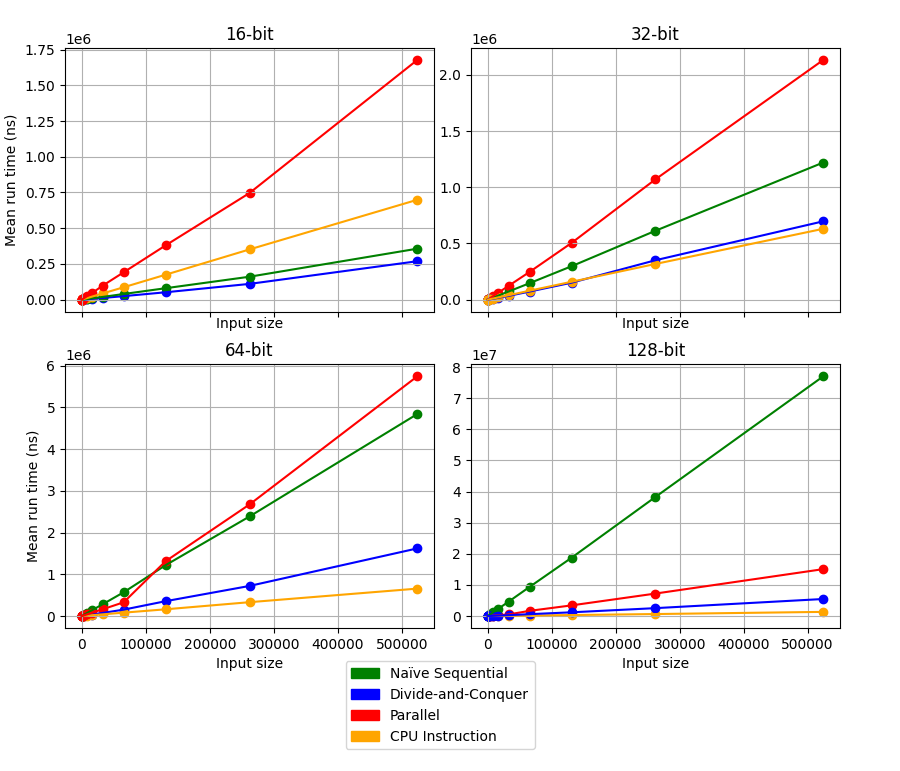
\includegraphics[width=\textwidth]{combined.png}
    \caption{Execution time of each algorithm on different word-lengths}
    \label{fig:runningtime}
\end{figure}
The benchmarks were run on different input sizes that were all powers of two - in this case $\{2^4, 2^5, \dots 2^{19}\}$ and with word sizes $\{16, 32, 64, 128\}$. The results can be seen in figure \ref{fig:runningtime}. 
It can be seen that the parallel algorithm is significantly slower for small word sizes, and only becomes more efficient than the naïve sequential algorithm when $d=128$. This must mean that the hidden factors hidden in the big-O notation of the parallel algorithm's time complexity outweigh the $d$ factor of the naïve algorithm. This makes sense, since the parallel algorithm is much more complex and only starts benefitting from parallelism after the first three iterations. Interestingly enough, when $d=64$, the parallel algorithm only seems to be slower when the input size is larger than $2^{16}$. This can be due to the input data being able to fit inside 128 KiB Li1 data cache on my machine (see appendix A for machine specifications).\\
When run on 128-bit size words, the naïve sequential algorithm performs much worse than than both the parallel and the divide-and-conquer algorithm. This shows that when we increase the word size, algorithms that have a linear dependency on $d$ suffer much more than algorithms that have a logarithmic dependency, which is as expected.\\
It is also seen that the divide and conquer algorithm significantly outperforms both the parallel and the naïve algorithm at all word sizes. This is might be due to the fact that it is much simpler than the parallel algorithm and is asymptotically more optimal than the naïve sequential algorithm.
The final thing to note is that the \texttt{popcnt} CPU instruction is the ultimately fastest option out of the algorithms. This shows that these algorithms might only be useful on hardware that does not support this instruction or on very large wordsizes. Even then, the divide-and-conquer algorithm seems to be sufficiently efficient for many uses or even superior to the parallel algorithm despite its suboptimal theoretical running time.\\


% Er mine resultater signifikante?
% Er der overensstemmelse af den teoretiske analyse og de praktiske resultater?
% Kan vi be- eller afkræfte vores hypoteser?
% Er der nogle mulige fejlkilder som kan have påvirket resultatet?
% Hvad er der af usikkerheder i benchmarkingen?
% Hvad kan vi fortælle omkring virkeligheden? Hvem vil have nytte af disse resultater?
\subsection{Discussion}
% Det er svært at komme med nogle super gode konklusioner omkring ordstørrelsens påvirkning på køretiden da jeg kun kunne køre med to forskellige ordstørrelser på min PC
Even though the results indicate a clear advantage to simpler algorithms to perform bit counting, the parallel bit counting algorithm should not be completely dismissed. While we can be pretty sure that a smaller $d < w$ might not improve the performance of the parallel bit-counting algorithm compared to the other algorithms, we do not know how the parallel algorithm performs on very large word-sizes (e.g. 256 to 384 bit words) as seen on some GPU units\cite{techpowerup}. Since the applications of the similarity search problem usually apply to very large data sets, it is often appropriate to perform highly efficient parallel calculations when possible. 
Parallel programming comes with many new challenges that were not considered in this project such as minimizing read/write operations to the main memory of the computer, the memory capacity of the graphics card and the size of the register files. 
This makes an actual implementation of the algorithm \ref{alg:parallel-d-and-c} non-trivial, especially since most programming interfaces for interacting with a GPU relies on intricate low-level systems programming (unless one were to use a language like Futhark\cite{futhark}). A nice feature of the algorithm is that it does not use multiplication, which means that many of the computations might be efficiently computed on a GPU.\\
Another thing that this experiment does not take into account is the index calculation time required to actually look up into the list of cardinalities. This was not included, since the correctness criteria of the algorithm may or may not take into account whether or not the cardinalities should have the same index in the final list as the input data.\\
The implementation that this experiment relied upon was optimized as per the best of my abilities, but futher optimizations might be possible. A nice feature of the Rust programming language is that the time complexity is very often documented in the documentation, which was very useful when working with heap-allocated vectors of numbers. The implementation was also written to be as generic as possible in regards to word size such that the experiment would be performed as unbiased as possible. This was possible due to Rust's generics, and while Rust design philosphy relies upon zero-cost abstractions\cite{rust-lang} (like C++), this might cause some optimization issues. Further optimizations might also be possible by manually analyzing the produced assembly code, which was regarded as out-of-scope for this project.\\
In general, while parallel bit counting theoretically is more efficient than its sequential and instruction-level counterparts, it has yet to be shown to be the case in practice. While further research might research how it performs on specialized hardware, the algorithm behind this will probably first be useful when larger word-sizes become more easily available and computable, if ever.

% Vi foretog indgående analyse af eksisterende løsninger på Approximate SS problemet, der viste at advancerede teknologier som præsenteret af Dahlgaard et al. osv er teoretisk overlegende hvis man er villig til at foretage nogle specifikke tradeoffs.
% En praktisk implementation viste sådan og sådan med denne specificitet ud fra sådanne benchmarks.
% Vores konklusioner er bla bla, og det indikerer bla bla.
% Ydergående undersøgelser kan undersøge ligende og lignende.
\section{Conclusion}
An in-depth analysis of existing solutions to the Approximate Similarity Search Problem described how many existing solutions utilize sketching to achieve a low query time with a constant error probability. In the case that one wants a sub-constant error probability, a possible solution by \citet{fast-similarity-search} was presented that can reduce the query time even further.

An important part of this optimization relies in being able to quantify the accuracy of a collection of data structures very efficiently, which is done in part by calculating the cardinality of a sequence of bit-strings packed into a list of words. \citet{fast-similarity-search} presents an algorithm to do this in parallel, which reduces the total query time to be sub-linear to the amount of sets in the corpus.\\
An analysis of the bit-counting algorithm shows its correctness with a few modifications alongside a theoretical running time which matches \cite{fast-similarity-search}. Benchmarks performed on an actual implementation tells otherwise however, showing that the word parallelism used to achieve a low amortized cost actually is hard to match simpler algorithms in practice when used on standard word sizes. Further research might focus on benchmarking the algorithm on more specialized hardware, although rewriting the implementation seems to be non-trivial.

\section{Appendices}
\begin{appendices}
\setcounter{secnumdepth}{2}
\renewcommand\thesubsection{\Alph{subsection}}
\subsection{Machine Specifications}
\label{appendix:machine-specs}
\begin{table}[H]
\begin{tabular}{ll}
\hline
\multicolumn{1}{|l|}{Model}            & \multicolumn{1}{l|}{Lenovo Thinkpad E580}                        \\ \hline
\multicolumn{1}{|l|}{Operating System} & \multicolumn{1}{l|}{Arch Linux kernel 5.15.5-arch1-1}            \\ \hline
\multicolumn{1}{|l|}{Word size}        & \multicolumn{1}{l|}{64bit}                                       \\ \hline
\multicolumn{1}{|l|}{Processor model}  & \multicolumn{1}{l|}{Intel(R) Core(TM) i7-8550U CPU @ 1.80GHz}    \\ \hline
\multicolumn{1}{|l|}{ISA}              & \multicolumn{1}{l|}{x86\_64}                                     \\ \hline
\multicolumn{1}{|l|}{Memory Capacity}              & \multicolumn{1}{l|}{32 GB}                                     \\ \hline
\multicolumn{1}{|l|}{Caches}           & \multicolumn{1}{l|}{128 KiB L1d, 128 KiB L1i, 1MiB L2, 8 MiB L3} \\ \hline
                                       &                                                                  \\
                                       &                                                                  \\
                                       &                                                                  \\
                                       &                                                                  \\
                                       &                                                                  \\
                                       &                                                                  \\
                                       &                                                                 
\end{tabular}
\end{table}

\subsection{Code}
\label{appendix:code}
The code for the implementation part can be found on in this Github repository: \url{https://github.com/Snailed/parallel-bit-counting}.
\end{appendices}


\printbibliography
\end{document}
